\section{Stage-Resolved Memory Transport}
\label{sec:mechanism}

\begin{figure}[t]
\centering
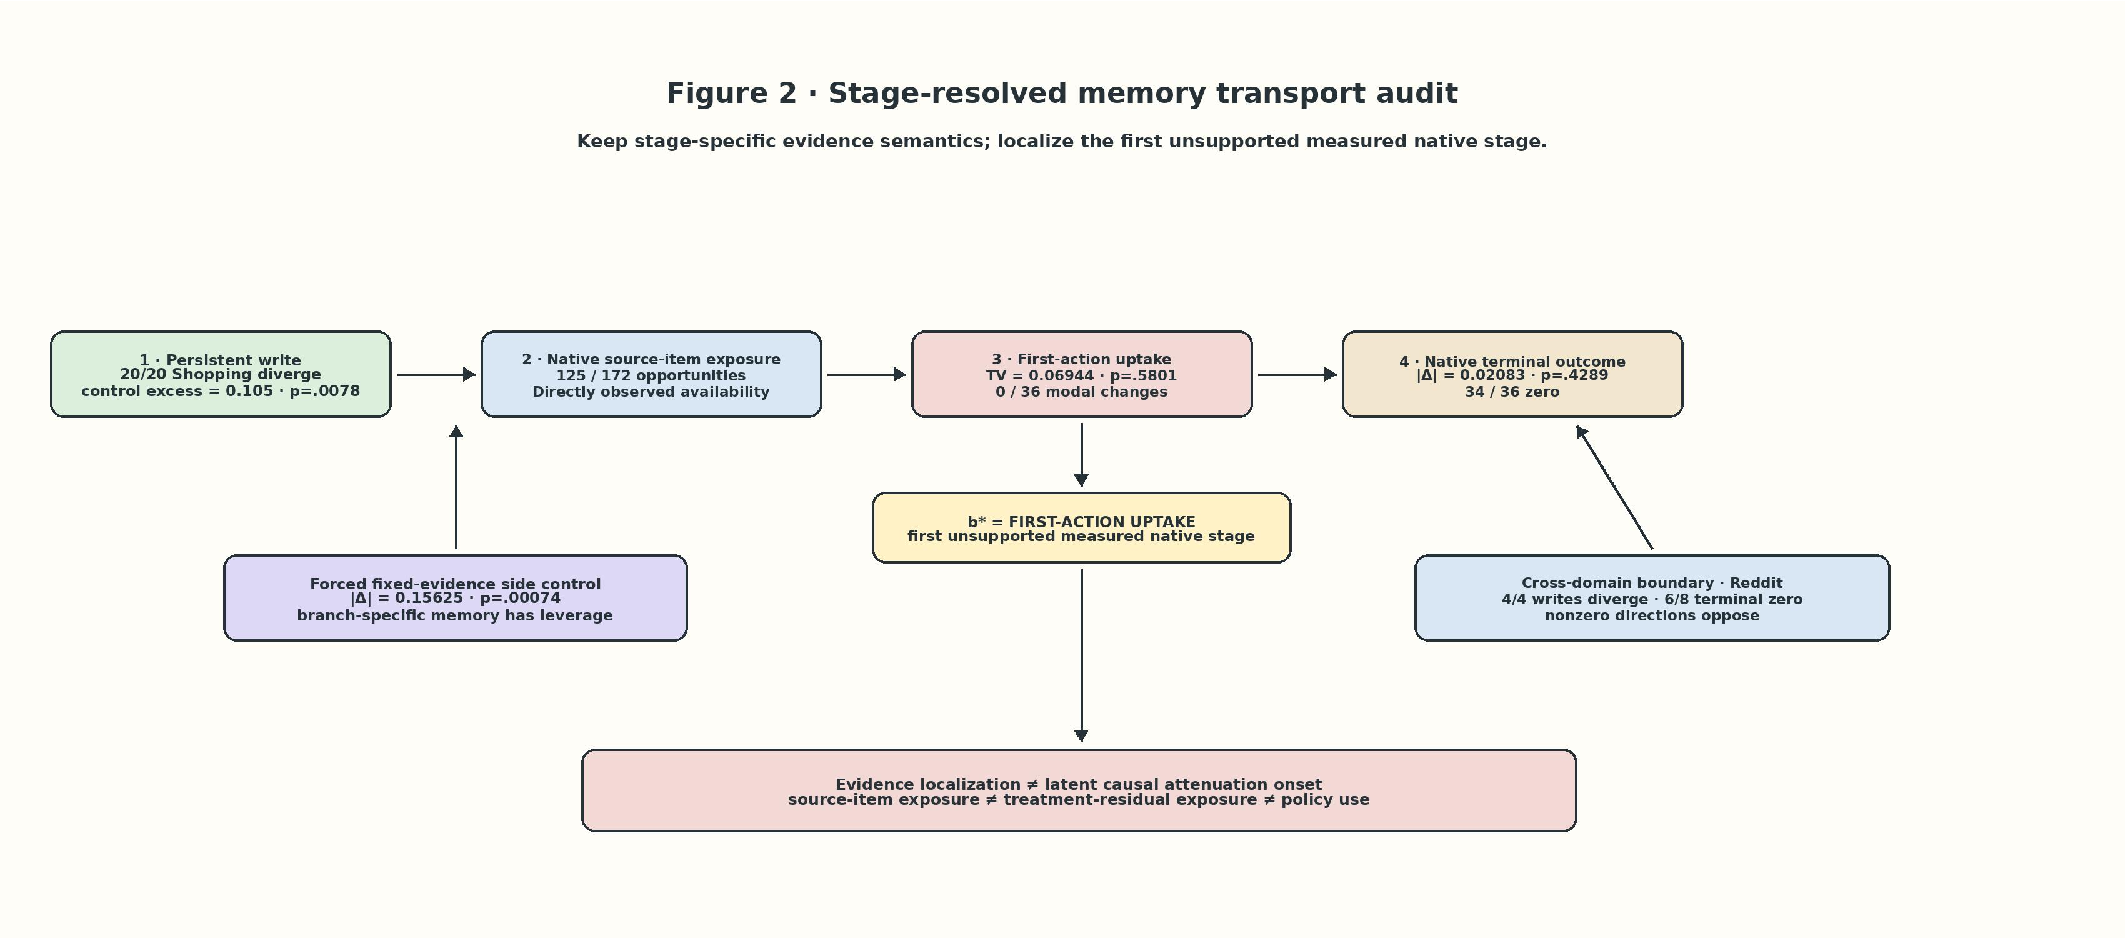
\includegraphics[width=0.99\linewidth]{figures/c1-stage-transport-method-handdrawn.pdf}
\caption{\textbf{Method: preserve stage-specific evidence semantics instead of collapsing memory reuse into one score.} The native path is persistent write $\rightarrow$ source-item exposure $\rightarrow$ first-action uptake $\rightarrow$ terminal outcome. On the frozen Shopping tests, write is supported, item exposure is directly observed, and first-action uptake is the first measured native stage whose branch contrast is not supported; terminal differences are sparse. Forced fixed-evidence exposure is a side capacity control that bypasses native retrieval, while Reddit supplies a cross-domain boundary on write-versus-terminal transport. The evidence boundary $b^*$ is ordinal: it is not a latent causal attenuation onset, and source-item exposure is not treatment-residual exposure or policy use.}
\label{fig:c1-method}
\end{figure}

\subsection{Controlled write intervention}
Let $\tau$ denote a frozen interaction trajectory before persistent memory construction. We create two writer conditions on the same $\tau$,
\[
  r\in\{S,F\}, \qquad m^{(r)} = g(\tau,r),
\]
where $g$ is the released memory writer and $S/F$ selects its success- or failure-reflection mode. The operational write contrast is
\[
  W(\tau)=d_{\mathrm{mem}}\!\left(m^{(S)},m^{(F)}\right).
\]
$W>0$ establishes that the frozen writer produced different persistent states. It does \emph{not} establish that every textual atom is a pure causal effect of the reward bit, because decoding randomness is not separately noise-calibrated at the atom level. We therefore use the same-mode wording control in Section~\ref{sec:prompt-control} to test the stronger alternative that ordinary prompt wording alone explains the observed write divergence.

\subsection{Native transport is a sequence of distinct observables}
For a held-out future query $q$, define native retrieval exposure at the source-item level,
\[
 E_r(q)=\mathbf{1}[m^{(r)}\in\operatorname{Retrieve}(q;\mathcal{M}^{(r)})].
\]
Exposure is an availability variable: it says that the branch-conditioned source-memory item reached the policy context. It does not identify which treatment-specific content inside that item was read or used by the policy. In particular, source-item exposure is weaker than \emph{treatment-residual exposure}: the latter would require showing that the branch-differentiating content, rather than merely the shared source item, is represented in the policy's effective readout. The frozen logs support the former but do not identify the latter.

We therefore measure the first downstream decision boundary separately. Let $p_r^{(1)}(\cdot\mid q)$ be the empirical distribution over the normalized first structured action emitted under branch $r$ for the same matched future-task state. The support is the set of first structured actions observed in either branch for that state; actions absent from one branch receive zero mass there. The action-level contrast is
\[
 U(q)=\operatorname{TV}\!\left(p_S^{(1)}(\cdot\mid q),p_F^{(1)}(\cdot\mid q)\right).
\]
Finally, for terminal outcome $y_r(q)$,
\[
 O(q)=\left|y_S(q)-y_F(q)\right|.
\]
A \emph{branch-comparison state} throughout the paper means one matched future-task state evaluated under the paired success- versus failure-conditioned memory branches while the non-memory task state is held fixed. The reported 36 Shopping states are 36 such matched comparison units; they are not 36 independent source trajectories.

The native scientific object is therefore the ordered observation tuple
\[
 \mathcal{T}_{\mathrm{native}}(q)=\big(W, E, U, O\big),
\]
not any one component in isolation.

Crucially, these components are \textbf{not commensurate}. $W$ is a memory-state distance, $E$ is an exposure indicator/rate, $U$ is a distributional action distance, and $O$ is an endpoint contrast. We therefore do not divide them into a scalar ``transport efficiency'' or treat their numerical differences as a mediation decomposition. The order is mechanistic; the scales are not.

A further identifiability issue is \emph{evaluation coarsening}. Let $\Pi_A(\mathcal{T}_{\mathrm{native}})$ project the chain onto observed stages $A\subseteq\{W,E,U,O\}$. The projection is many-to-one: for example, a small endpoint under $\Pi_{\{O\}}$ is compatible with writer failure, retrieval absence, post-retrieval filtering, or sparse heterogeneous transport, while $\Pi_{\{E\}}$ cannot distinguish availability from policy uptake. We therefore retain the categorical stage signature $\Sigma=(z_W,z_E,z_U,z_O;z_F)$, with $z_F$ denoting the forced-capacity side control. It is not a scalar metric; it preserves which explanations remain distinguishable after each stage is observed.

\subsection{Forced leverage is a capacity control, not a native stage}
The forced fixed-evidence experiment mechanically supplies paired memory content to the downstream task packet. Let
\[
 L_{\mathrm{forced}}(q)=\left|y^{\mathrm{forced},S}(q)-y^{\mathrm{forced},F}(q)\right|.
\]
Because native retrieval is bypassed, $L_{\mathrm{forced}}$ is not inserted between $W$ and $E$. It answers a different question: \emph{can} branch-specific memory content affect the downstream system when supplied? Native $(E,U,O)$ asks whether the deployed memory path \emph{does} transport that contrast. This capacity-versus-transport separation is the key control that prevents a weak native endpoint from being summarized as ``memory can never matter.''

\subsection{An ordinal stage-evidence ladder}
\label{sec:evidence-ladder}
The central measurement problem is that $W$, $E$, $U$, and $O$ cannot be compared on one numerical scale, and their frozen tests do not have matched sample units or statistical power. We therefore localize an \emph{evidence boundary} with an ordinal ladder rather than a post-hoc transport coefficient or a latent bottleneck estimator. Let the ordered native stages be
\[
  s_1=\text{write},\quad s_2=\text{retrieval exposure},\quad s_3=\text{first-action uptake},\quad s_4=\text{terminal outcome}.
\]
For each stage we preserve its native evidence semantics. A stage may be \textsc{Supported} by its frozen inferential test, \textsc{Observed} directly when the claim is descriptive rather than thresholded, or \textsc{Not-Supported} when its frozen primary test does not establish a stable branch contrast. We then define
\[
  b^*=\min\{j:\;s_j\text{ is not supported/observed while }s_1,\ldots,s_{j-1}\text{ are supported/observed}\}.
\]
This is an ordering rule, not a ratio: no cross-stage units are divided, normalized, or interpreted as mediation mass. Because the stage tests are not power-matched, $b^*$ means ``first unsupported measured stage under the frozen tests,'' not ``the stage where the true causal effect first becomes small.''

The forced fixed-evidence arm is evaluated separately as a \emph{side capacity condition}. It can weaken the global-insensitivity explanation, but because it bypasses native retrieval it cannot make an otherwise unsupported native stage pass. This prevents the positive forced endpoint from being inserted into the native chain merely because it is statistically strong.

\paragraph{Multiplicity and interpretation.} The frozen tests answer different stage-specific questions and are not searched as a family for the smallest $p$-value. We therefore do not make an omnibus ``at least one stage is significant'' discovery claim and do not use a post-hoc multiplicity correction to choose $b^*$. The boundary operator depends on the preregistered ordering and each stage's own frozen evidence rule. Reported $p$-values should consequently be read as stage-local evidence summaries, not as interchangeable entries in a single multiple-testing family.

The same ladder can be read as an alternative-explanation audit:
\begin{align*}
\textbf{A1: no state intervention} &\Rightarrow W\approx 0,\\
\textbf{A2: global downstream insensitivity} &\Rightarrow L_{\mathrm{forced}}\approx 0,\\
\textbf{A3: retrieval absence only} &\Rightarrow E\approx 0,\\
\textbf{A4: exposure is uptake} &\Rightarrow \text{observed }E\text{ should be accompanied by supported }U,\\
\textbf{A5: universal directional transport} &\Rightarrow O\text{ should be broadly nonzero with stable sign.}
\end{align*}
In our frozen evidence, write is \textsc{Supported}, native source-item exposure is \textsc{Observed}, first-action uptake is \textsc{Not-Supported}, and terminal transport is sparse and sign-heterogeneous. Hence $b^*=s_3$: \textbf{first-action uptake is the first unsupported measured native stage after write and source-item exposure have been established}. The positive forced side control further weakens a global-insensitivity account without changing $b^*$; it does not identify a native latent attenuation onset.

This is still not an identified mediator coefficient. A causal mediation statement would additionally require compatible intervention surfaces and a noise/seed design that isolates each branch-specific atom. We do not have that evidence and do not make that claim.

\subsection{Interpretation discipline}
For clarity, we use four terms narrowly: \textbf{write} means that the persistent state changes; \textbf{exposure} means that the branch-conditioned source item appears in native retrieved context; \textbf{uptake} means that a measured policy decision distribution changes across branches; and \textbf{capacity} means that supplied branch-specific memory can affect downstream behavior when native retrieval is bypassed. These are measurements on different surfaces, not synonyms for ``memory use.''

Three non-implications are load-bearing throughout the paper:
\[
  \text{persistent-state divergence}\not\Rightarrow\text{behavioral divergence},
\]
\[
  \text{retrieval exposure}\not\Rightarrow\text{policy uptake},
\]
\[
  \text{forced leverage}\not\equiv\text{native end-to-end transport}.
\]
These distinctions also explain why our stopped evidence-gated residual extension is not a negative method result: that extension failed qualification before a behavioral method-effect experiment was authorized. The present paper therefore remains an identification/measurement study of the transport chain.
